
\documentclass[Master.tex]{subfiles}
\begin{document}
\begin{frame}
\begin{figure}
\centering

\includegraphics[width=1.05\linewidth]{images/StatsBase-ScreenShot}

\end{figure}


\end{frame}
%===================================%
\begin{frame}
\begin{figure}
\centering
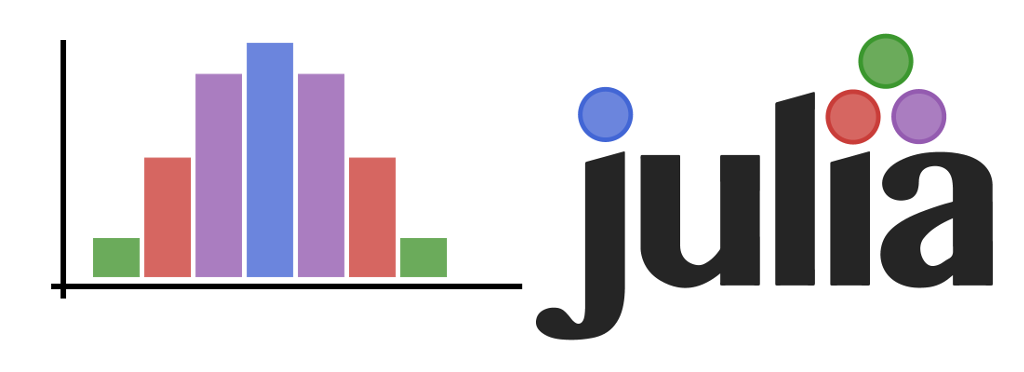
\includegraphics[width=0.4\linewidth]{images/statsbase-logo}

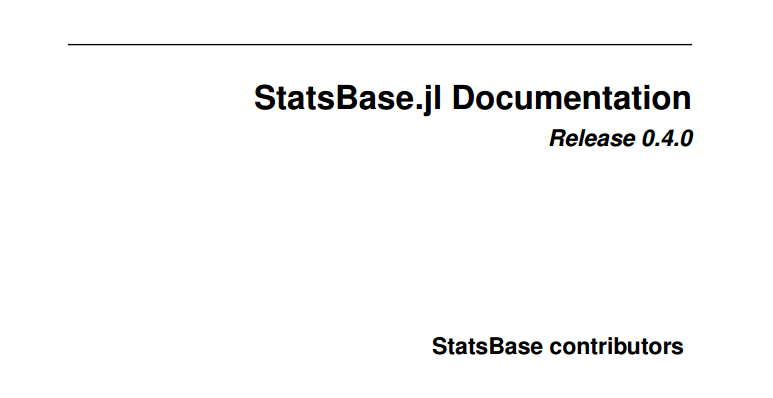
\includegraphics[width=0.8\linewidth]{images/statsbase-docs}

\end{figure}

\end{frame}
\begin{frame}[fragile]
\frametitle{Statistics with Julia}	
\large
\noindent \textbf{StatsBase.jl}
\begin{figure}
	\centering
	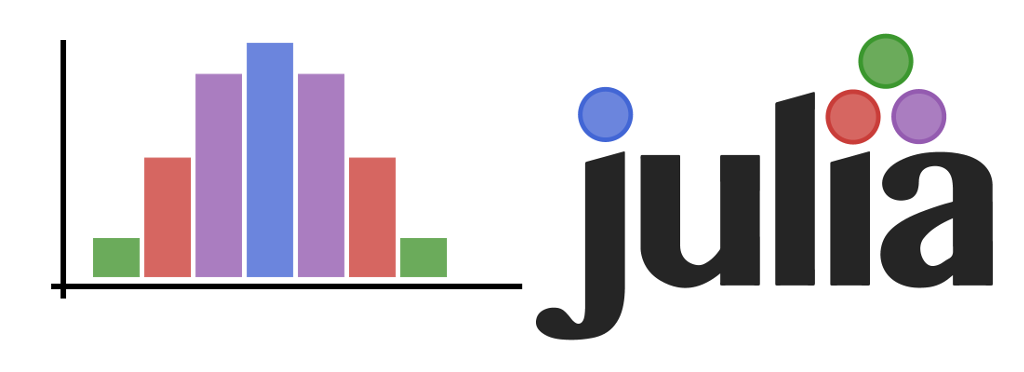
\includegraphics[width=0.4\linewidth]{images/statsbase-logo}
	
\end{figure}
\begin{itemize}
	\item StatsBase.jl is a Julia package that provides basic support for statistics. 
	\item Particularly, it implements a variety of statistics-related functions, such as scalar statistics, high-order moment computation, counting, ranking, covariances, sampling, and empirical density estimation.
\end{itemize}
\end{frame}
%=============================================%
\begin{frame}[fragile]
	\frametitle{Statistics with Julia}	
	\large
\vspace{-1.5cm}
Measure of Centrality :  Who am I?\\ \bigskip
{
	\LARGE
\[ \frac{Q_1 + 2Q_2 + Q_3}{4} \]
}
	
\end{frame}
\end{document}